%% The following is a directive for TeXShop to indicate the main file
%%!TEX root = diss.tex

\chapter{The \toolname{} Plugin}
\label{ch:Tool}

\begin{epigraph}
  \emph{Mitochondria is the powerhouse of the cell}\\
     ---~Anonymous
\end{epigraph}

\noindent \toolname{} is an open-source\footnote{\url{https://github.com/jyoo980/reach-hover}}
plugin developed on the JetBrains IntelliJ Platform.
Section \ref{sec:DesignMeth} discusses the design methodology for \toolname{},
derived from the data presented in Chapter \ref{ch:Survey} and an investigation
of current tools that provide information that might be used to help answer
reachability questions.
In section \ref{sec:UsingReachHover}, we describe how a user might use
\toolname{} in a software development scenario, with a particular focus on
its mechanism of invocation and how it visually presents data.
The implementation of \toolname{} is detailed in section
\ref{sec:Impl}.

\section{Design Methodology}
\label{sec:DesignMeth}

\noindent To inform the design of \toolname{}, we analyzed the data from a 
survey that sought to identify the type and frequency of reachability questions 
that are asked by software developers in practice.

Figure \ref{fig:SurveyResults} shows that Development Questions 1, 2, 5, and 9
were the most frequently asked among our respondents.
Using Table \ref{Table:SurveyTags} to map these questions to their associated
tags, we found that $Q_{find}$ was the most frequent type of question asked out
of the top four ranked by our respondents.
Specifically, these questions were:

\begin{itemize}
  \item[] \textbf{Development Question 1}:\\ \textit{Where did a value come from,
  and/or how was it formed?}
  \item[] \textbf{Development Question 2}:\\ \textit{Given some data, which
  parts of it are modified downstream?}
\end{itemize}

\par We noted that these questions are thematically related. They are instantiations 
of the \textit{find} category of reachability questions, and they can also be
answered by traversing backward and forward in a data-flow trace, respectively.
For example, to answer Development Question 1, a user could invoke a backward
data-flow trace, and filter for nodes that have a control or data dependency
on the value under analysis.
The same analysis could be performed on a forward data-flow trace to answer
Development Question 2.
Consequently, we decided to build \toolname{} with a particular focus on
supporting these two questions for the sake of thematic coherence.

\par Since information provided from a data-flow trace could be used to answer
the questions we attempt to support with \toolname{}, we began by investigating 
existing data-flow analysis tools to obtain an understanding of the current 
landscape of analysis tooling.
The IntelliJ IDEA \ac{IDE} exposes forward and backward data-flow analysis
capabilities to users.
Figure \ref{fig:IntelliJDataflow} shows how a user might invoke a backward 
data-flow analysis, while the result of this analysis is shown in
Figure \ref{fig:IntelliJDataflowResult}.
We found these pre-existing data-flow capabilities to be a good basis for the 
development of \toolname{} due to its ease of extension via the JetBrains 
IntelliJ Platform \ac{SDK}.

\par Next, we began to identify pain points that users might face as they
invoked the data-flow analysis tool.
We observed that discovering the tool itself might be difficult for
users; the action to invoke the tool was a three-click action.
Additionally, the action was hidden behind a context menu that did not appear
to have a strong information scent that guided users to discovering and invoking
the tool from a very broad list of options (\ie data-flow-specific analyses
are accessed via a general ``Analyze" menu element).
In the result presented by the data-flow analysis tool, each element in the 
data-flow trace is presented as an node in a tree-like structure that is 
structurally similar to a conventional hierarchical tree.
We found this to be useful for preserving the structural information relevant
to our target reachability questions (\eg method calls \texttt{a} and \texttt{b}
within a method \texttt{c} are displayed as children of the node \texttt{c} in
the tree).

\par Although structural information was easily preserved through the tree, each node
displayed only the single line of code within the data-flow trace, often
without visual aids such as syntax highlighting.
This meant that users often analyzed each node in isolation from any surrounding
context, particularly if they were not aware that double-clicking a node in the
tree would focus the editor pane to the line of code under inspection.
However, this might introduce the additional problem of frequent context
switching and reconstruction as editor focus shifts between files and code
blocks.

\par Investigating the current tooling available for data-flow analysis, and
its associated user pain points provided a foundation for the design of 
\toolname{}.
We attempted to achieve the following with the design of our tool:

\begin{itemize}
  \item[] \textbf{Design Goal 1}: \\
    \textit{
      User friction should be minimized between the developer and \toolname{},
      especially with respect to how they might discover and invoke the tool.
    }
  \item[] \textbf{Design Goal 2}: \\
  \textit{
    \toolname{} should present more context surrounding a data-flow node in
      a way that minimizes the amount of context switching for a developer.
  }
\end{itemize}

We describe the user-facing result of implementing these goals in section
\ref{sec:UsingReachHover}, while a technical discussion of their implementation 
is discussed in section \ref{sec:Impl}.

\section{Using \toolname{}}
\label{sec:UsingReachHover}

In this section, we describe how a user might interact with \toolname{}, framed
within the context of a software development task.
First, we describe how a user might invoke our tool to begin the process
of answering a reachability question.
Next, we describe the user interface of the visualization presented by 
\toolname{}.

\subsection{Invocation Interaction}
\label{subsection:InvocationInteraction}

\noindent A task where a developer might want to use \toolname{} might be when 
they are investigating how a value was created, or where it originated in a 
data-flow trace. 
Work in information search and retrieval systems
\cite{huang-2012-mouse,guo-2010-hover} has provided empirical evidence that cursor
hovering might be a useful proxy for determining a user's focus or interest in
a user interface component.
We use this empirical evidence to inform our design of an invocation mechanism 
for \toolname{} that is based on cursor attention and hovering.

\par The initial invocation mechanism for \toolname{} is shown in Figure 
\ref{fig:ReachHoverInvokeBackward}.
In this figure, we assume a task where a developer is investigating the origin
of the value \texttt{editorKit}, which is an instantiation of 
Development Question 1.
The hover popup is shown containing two options; the first is to invoke
\toolname{} to begin a reachability analysis, and the second is to show the
documentation that is usually presented by IntelliJ IDEA when a user hovers
over a value.
This hover popup appears only only when a user hovers over a value after a 
certain delay that is commensurate with other user interface component delays 
in IntelliJ IDEA.
Due to the difficulty in overriding the default documentation popup that is
present in the \ac{IDE}, the reachability popup can sometimes appear in concert
with a documentation popup for a value.
We do not consider our interaction mechanism to be more intrusive than the
default data-flow analysis feature of the \ac{IDE};
a user would have had to right-click to select the value of interest and
navigate a context menu to invoke the analysis (Figure
\ref{fig:IntelliJDataflow}).
Furthermore, we attempted to address Design Goal 1 by presenting the ability to 
invoke \toolname{} directly on hover, rather than hidden under a number of 
context menus where user discoverability and friction might have increased.
It is also possible for the user to not use \toolname{} altogether, the default
context menus provided by IntelliJ IDEA are still available.
Another task where a developer might use \toolname{} is in exploring how a value
is modified or changed; Figure \ref{fig:ReachHoverInvokeForward} shows how
the hover popup appears in this case.

\begin{figure}[ht]
\centering
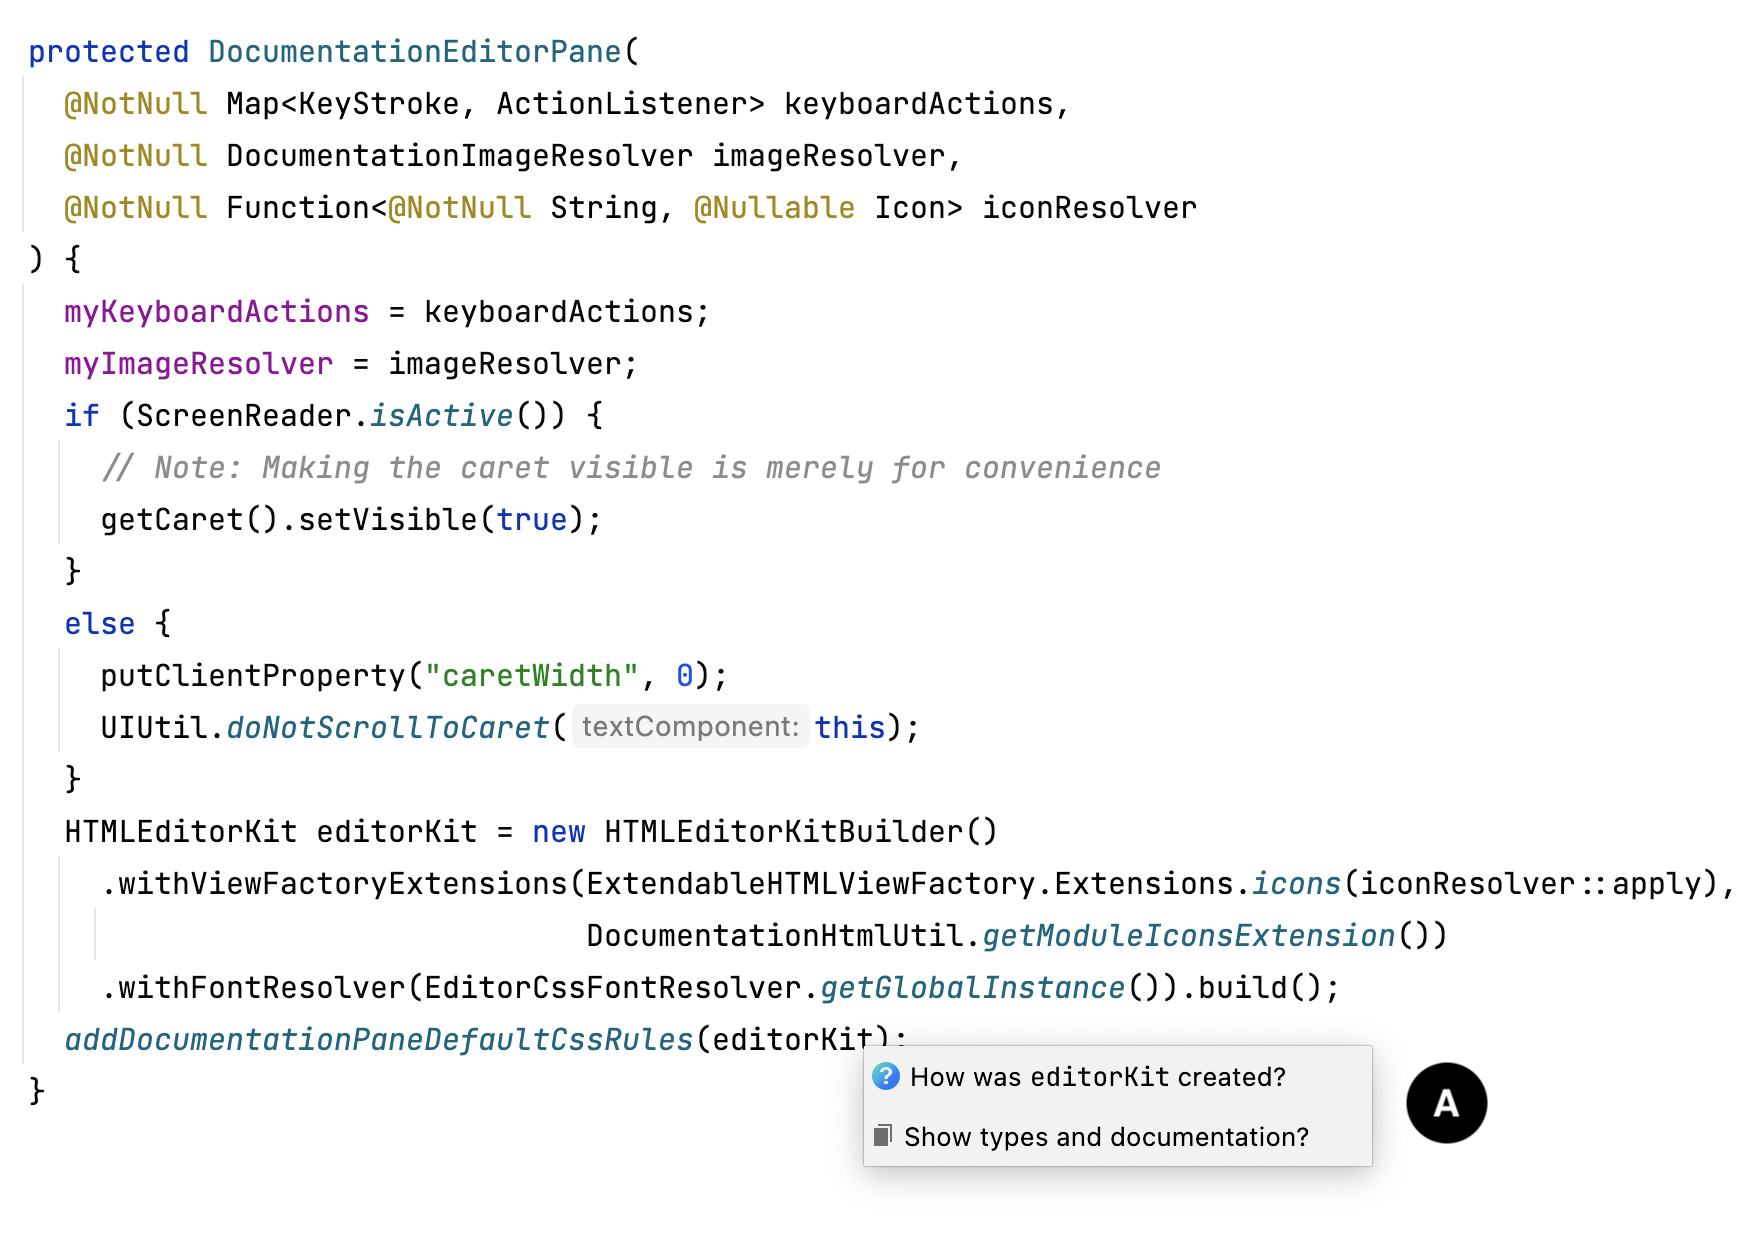
\includegraphics[width=\textwidth]{./figs/reach-hover-invoke.png}
\caption{
  The \toolname{} popup (A) that appears when a user hovers over a code
  structure of interest. In this case, \toolname{} poses the question:
  ``How was \texttt{editorKit} created?"
}
\label{fig:ReachHoverInvokeBackward}
\end{figure}

\begin{figure}[ht]
\centering
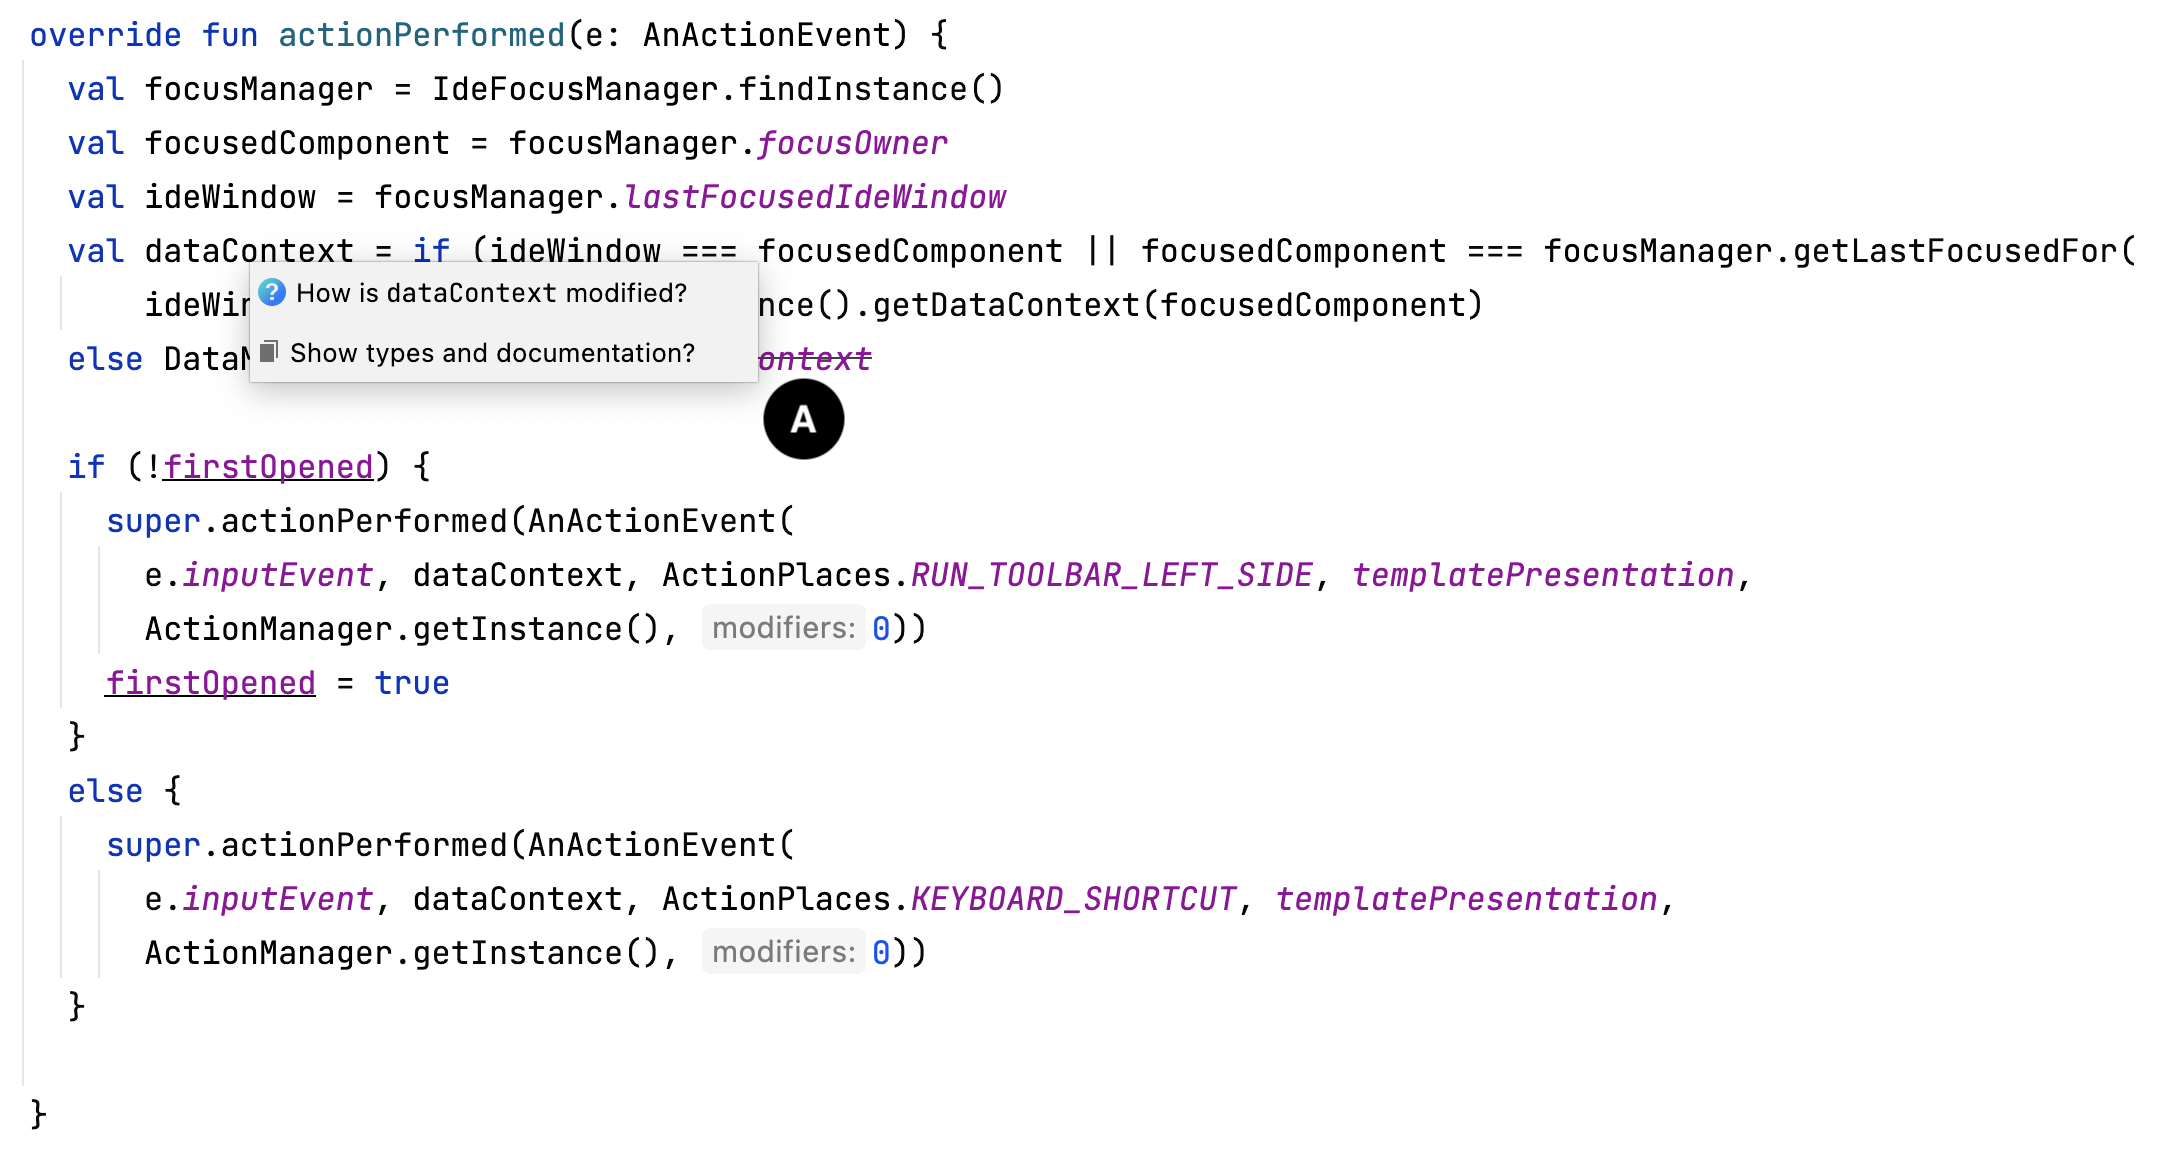
\includegraphics[width=\textwidth]{./figs/reach-hover-invoke-forward.png}
\caption{
  The \toolname{} popup (A) that appears when a user hovers over a code
  structure of interest. In this case, \toolname{} poses the question:
  ``How was \texttt{dataContext} modified?"
}
\label{fig:ReachHoverInvokeForward}
\end{figure}

\subsection{Result Visualization}
\label{subsection:ResultVisualization}

\noindent A goal of \toolname{} is to present more context surrounding the 
result of a data-flow analysis. 
We also wanted to preserve the structural information that was
already provided by existing static analysis tools, such as the data-flow
analysis tooling built into IntelliJ IDEA, or the call hierarchy explorer in
the Eclipse \ac{IDE}, which presents results using the same hierarchical
tree paradigm.

\par Preserving the presentation of structural information served two purposes.
First, we did not aim to completely redesign an interface for viewing data-flow
information;
our goal was to enrich an existing interface with additional information.
Introducing a completely new user interface paradigm might have introduced
additional complexity in the form of developers having to adapt to a new 
paradigm before our tool became useful to them.
Second, we wanted to preserve non-local context, \ie information that is not
directly observable from code and its surrounding context, such as how deep
within a call hierarchy a location in code exists.

\par We present the visualization component of \toolname{} in Figure
\ref{fig:ReachHoverVis}.
Information regarding a reachability question is presented in two main
sub-components.
High-level non-local context is provided in the top half of the main component,
which is the same component used by the the original data-flow analysis tool
built into IntelliJ IDEA.
Fine-grained local context is provided by the preview editor sub-component.
A developer is able to begin investigating code from a high-level by selecting
a row in the top component.
This triggers a change in the preview editor to focus on the line of code under
inspection, which is highlighted in its location in the editor.
Additional information, such as the file and project directory in which the
line of code under inspection is located, is presented in the bottom
toolbar of the main component.
Additionally, a user is able to select the scope of a reachability analysis
(\ie file, directory, and project-level) on-the-fly and without resorting to 
restarting the entire analysis from scratch, avoiding the need for expensive
context switching or reconstruction.
To the best of our knowledge, this is not a feature that is currently available
in the standard IntelliJ IDEA \ac{IDE}.

\begin{figure}[ht]
\centering
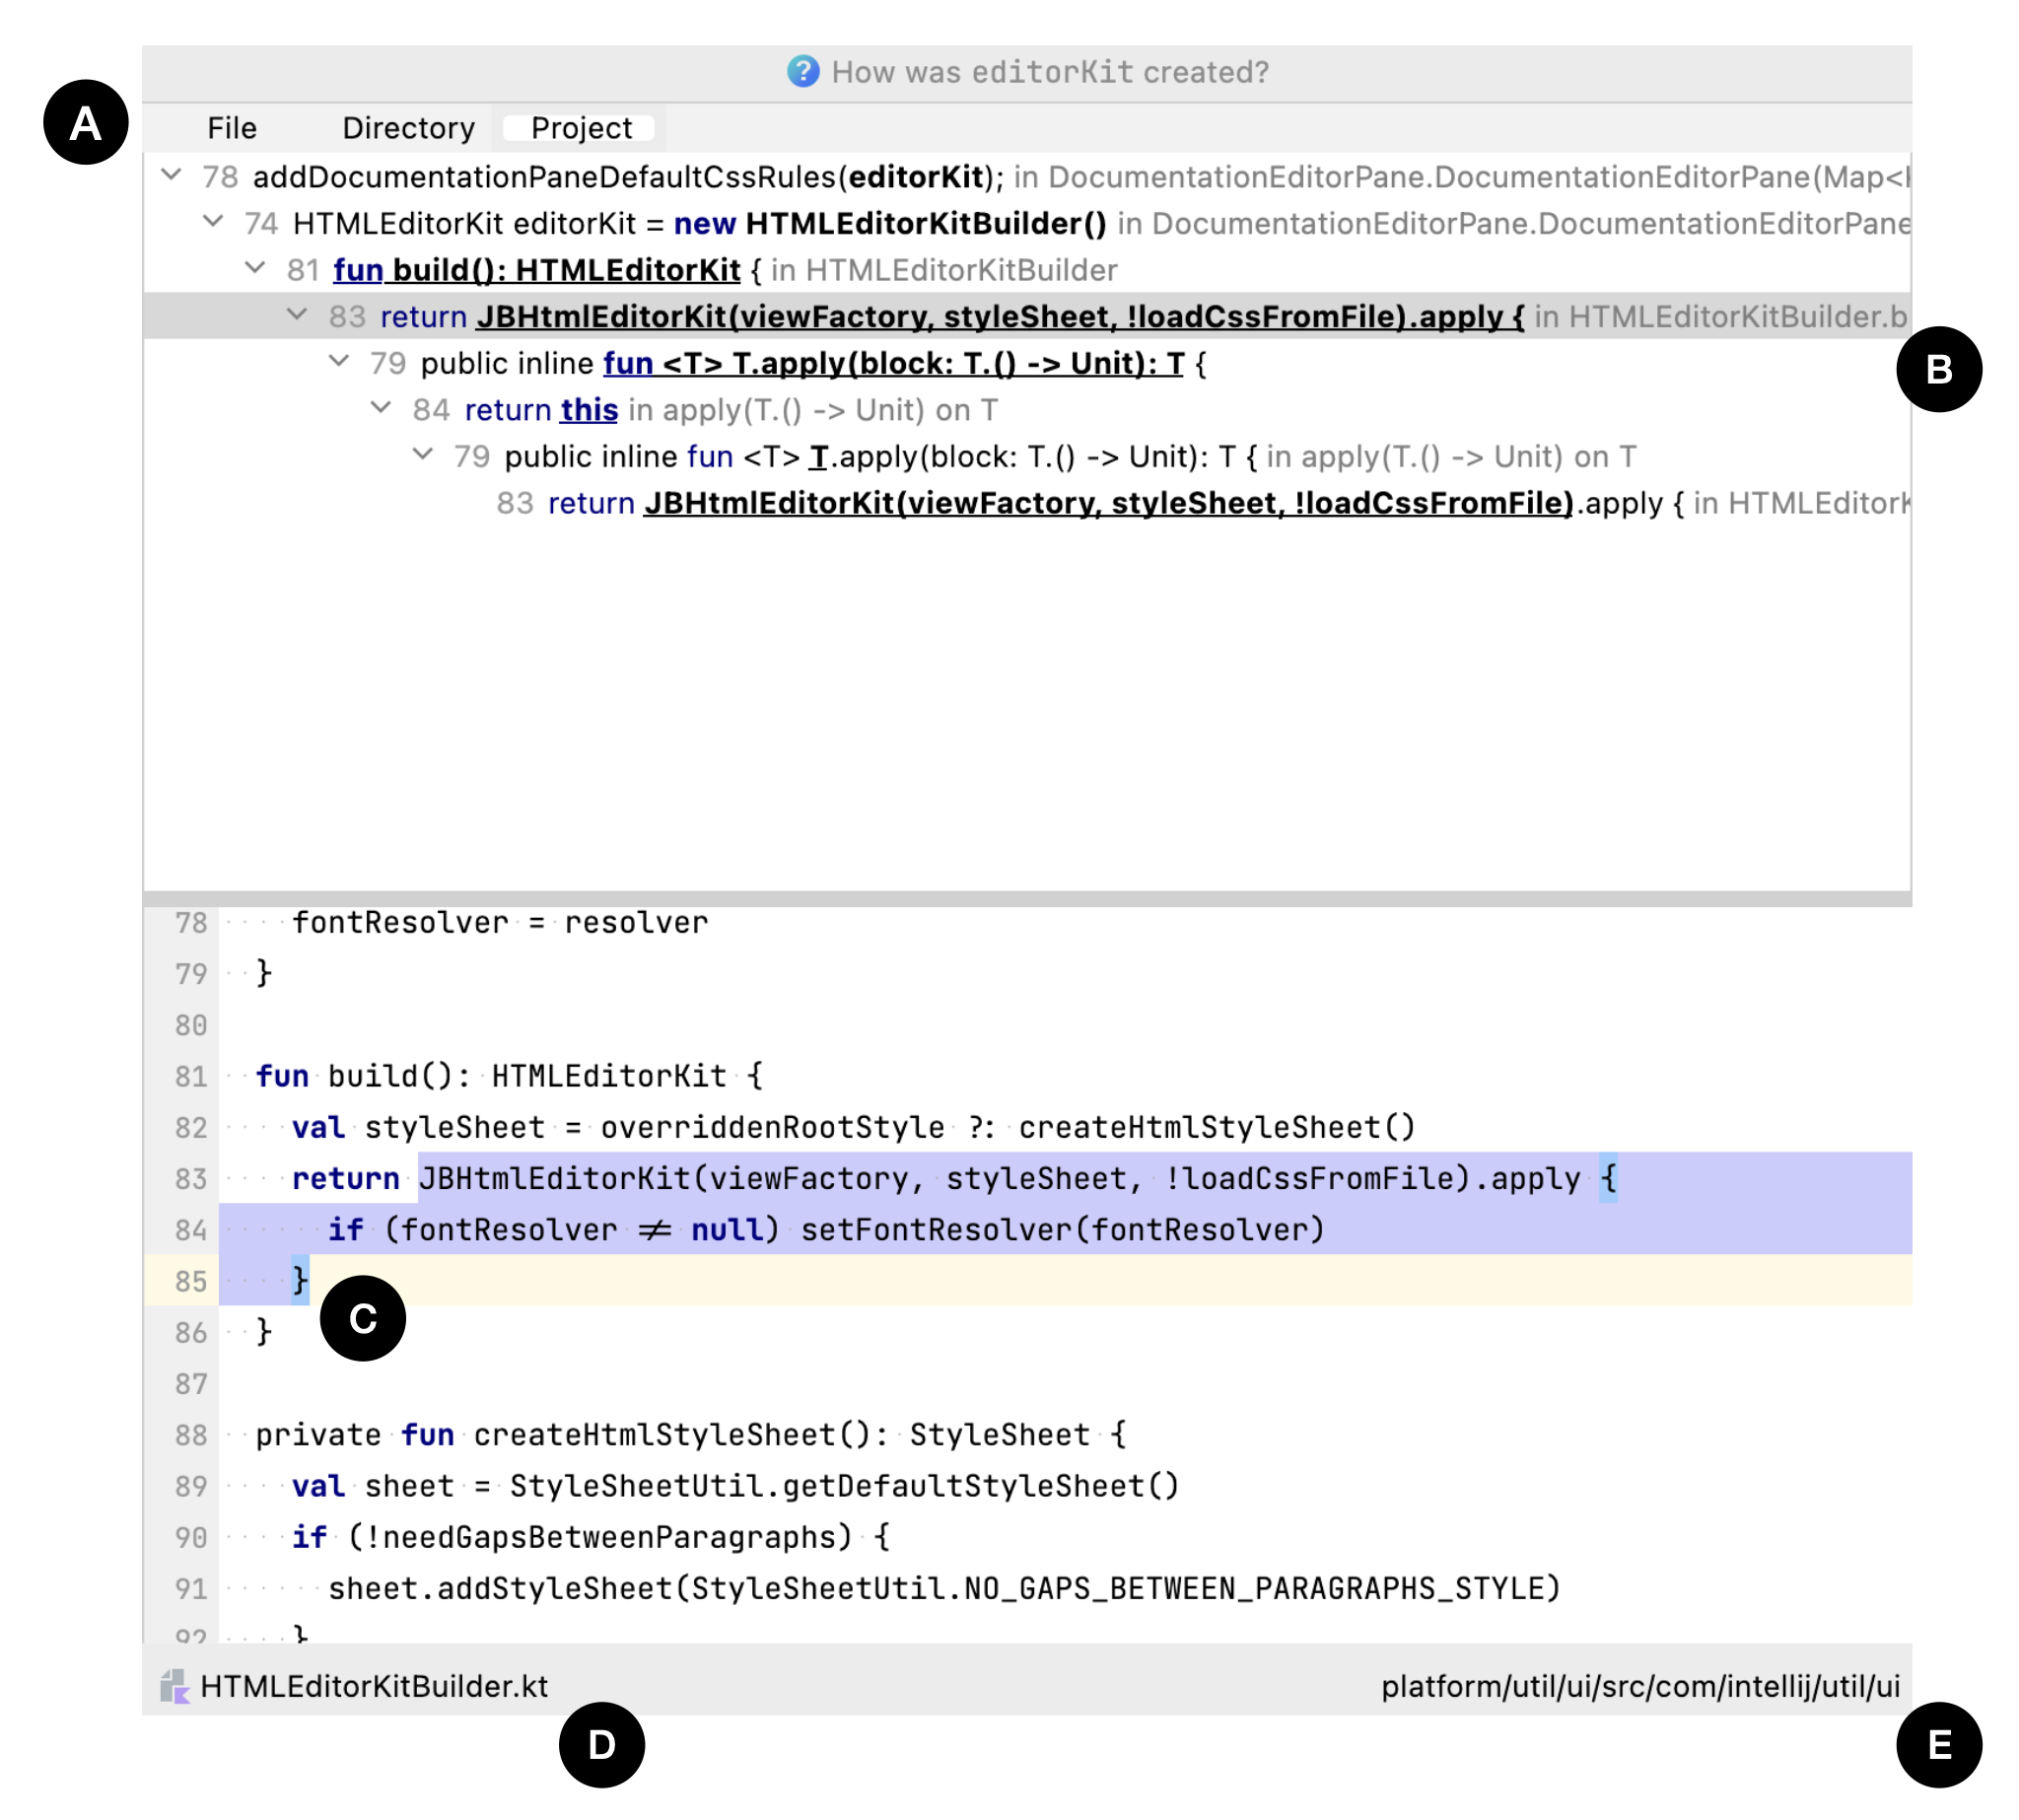
\includegraphics[width=\textwidth]{./figs/reach-hover-vis.png}
\caption{
  A data-flow trace presented by \toolname{}. (A) enables developers to select
  between a file, directory, or project-level scope for the reachability
  analysis. (B) contains the same hierarchical text-tree view as the standard
  IntelliJ data-flow analysis tool. (C) demonstrates the highlighting of the
  code under inspection that corresponds to the selected element in (B).
  The file name and directory are provided by (D) and (E).
}
\label{fig:ReachHoverVis}
\end{figure}

\section{Implementation}
\label{sec:Impl}

\toolname{} is implemented in the Kotlin programming language, and consumes
\acp{API} implemented in Java that are exposed by the IntelliJ Platform.
The implementation of \toolname{} can be separated into two main components:
a frontend and a backend.
The frontend detects cursor hover events and analyzes code for
reachability analysis viability, while the backend exploits existing data-flow
analysis features to visualize data for reachability analysis.

\subsection{Frontend: Detecting Values for Reachability Analysis}
\label{subsec:Frontend}

The \toolname{} frontend (Figure \ref{fig:ReachHoverFrontend}) is designed as 
a loosely-coupled component that aims to be largely orthogonal to a specific 
programming language or project structure.
We implement an existing event listener interface that is exposed by the
IntelliJ IDEA \ac{SDK} for public use in order to create a class that listens
for hover events in the editor (\texttt{EditorHoverListener}).
Whenever a code element is detected under a hover event, we call a utility 
class (\texttt{SliceDispatchService}) to determine whether a program slicer
is available for the code under inspection.
If a slicer is available, we convert the raw code element into a \ac{UAST} node.

\par The \ac{UAST} data type enables us to handle program elements in a
generalized manner. 
Consequently, the logic that determines whether an element is viable for
reachability analysis does not change across different programming languages.
The \ac{UAST} data type has support for programs written in Java or Kotlin.
We have extended the \ac{UAST} data type with two methods that enable us to
determine whether a given code element is a non-literal method argument, or
a local variable reference.
These specific code elements are candidates for the questions 
``Where did a value come from, and/or how was it formed?" or 
``Given some data, which parts of it are modified downstream?" respectively.

\par Using these methods, the \texttt{EditorHoverListener} dispatches a call to
the backend of \toolname{} to conduct either a forward or backward reachability
analysis by sending it a context object that contains the element under 
inspection, its location in the editor, and other metadata.

\begin{figure}[ht]
\centering
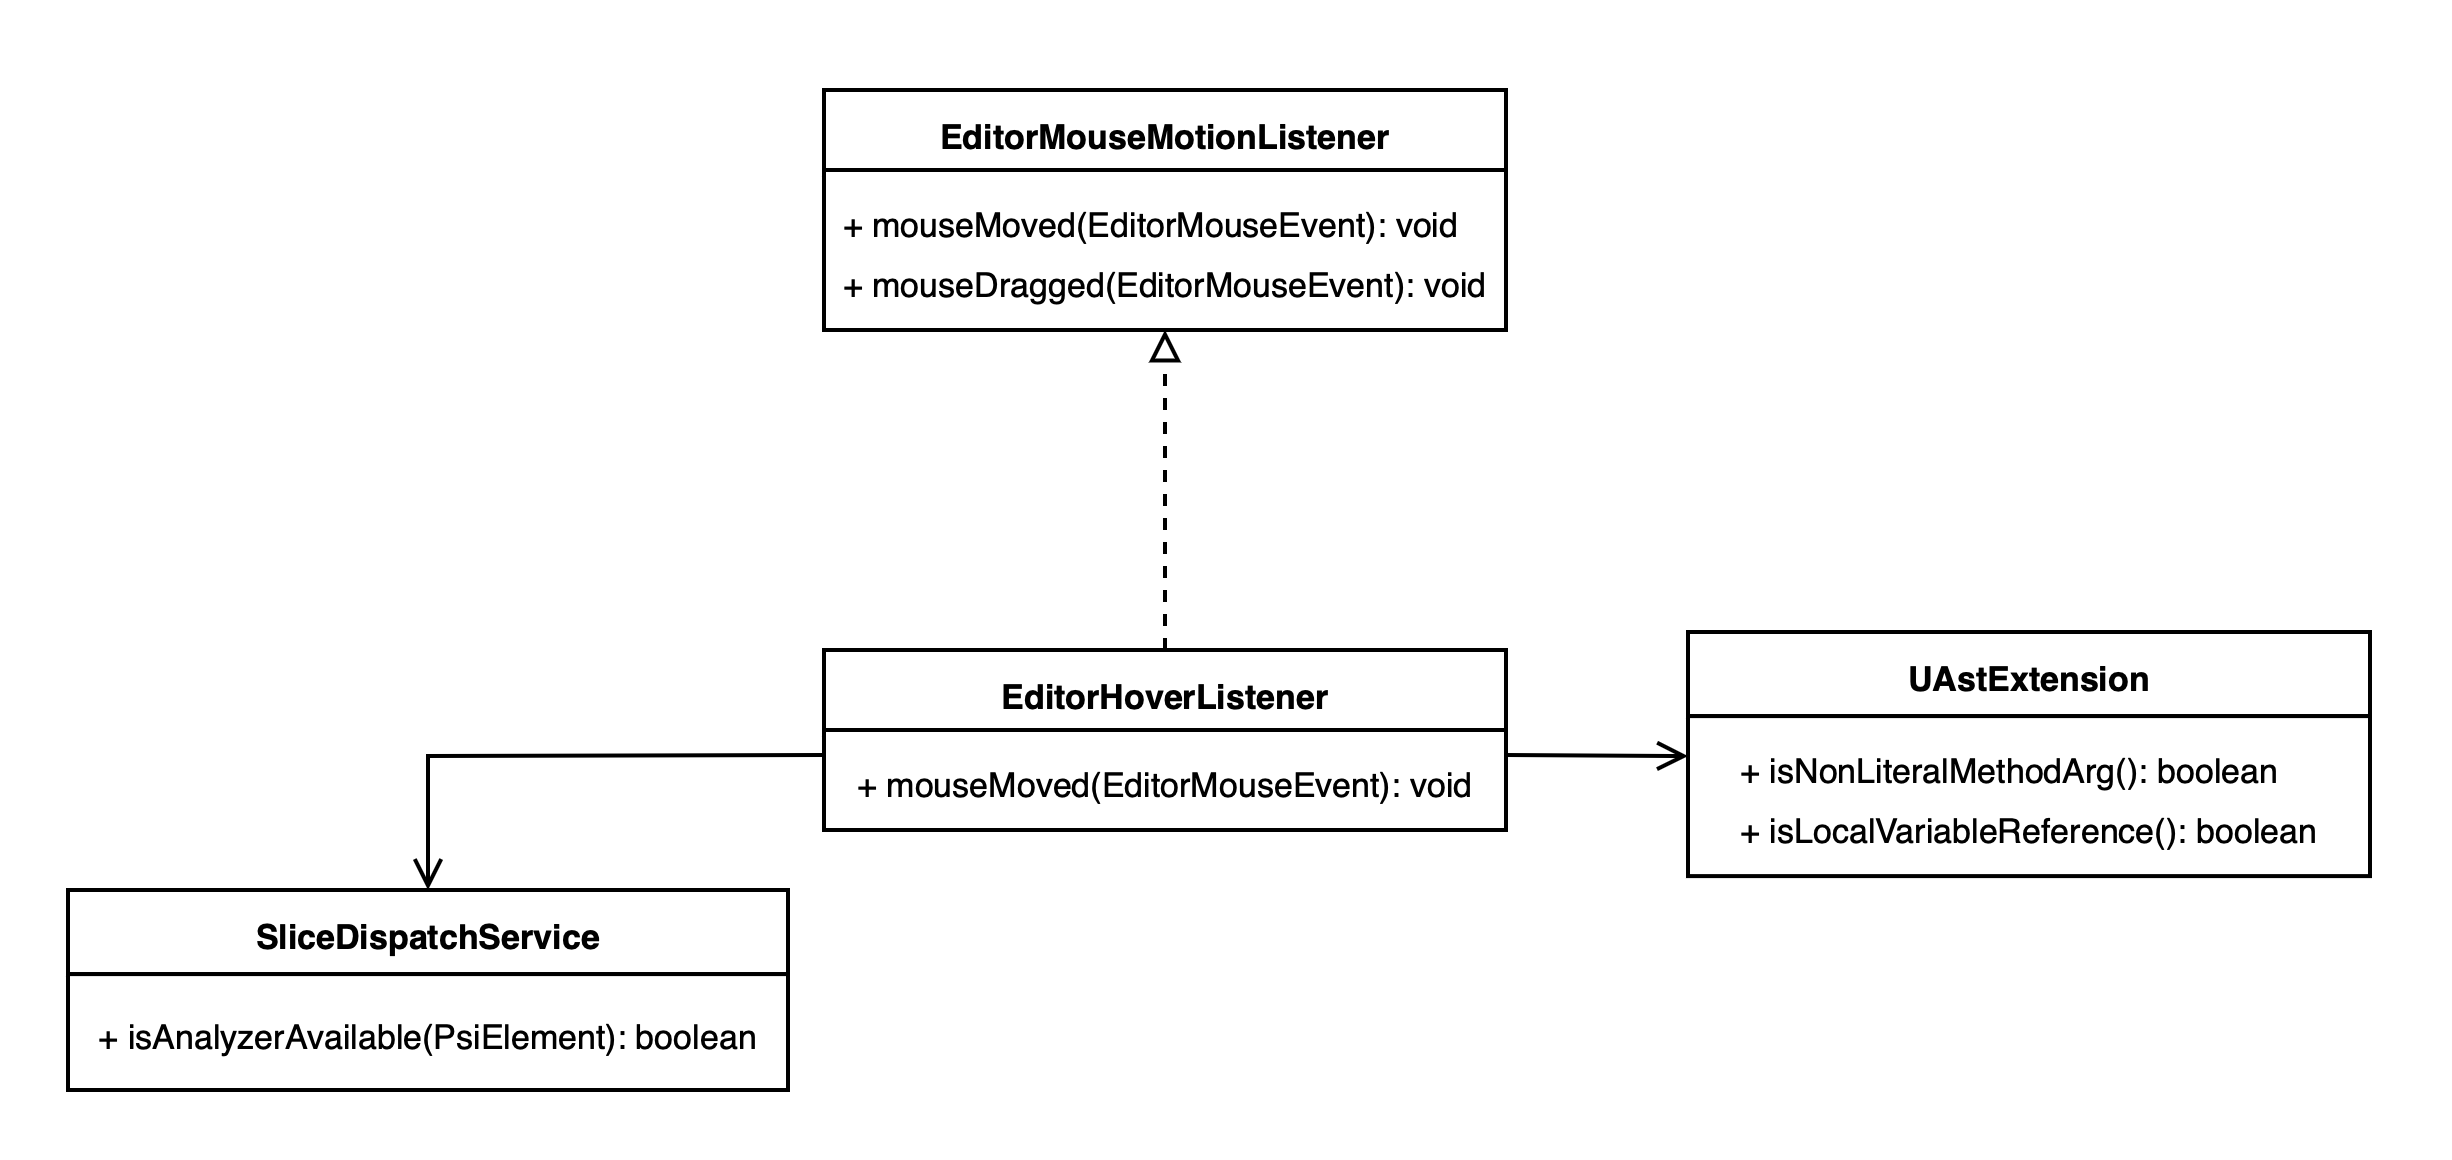
\includegraphics[width=\textwidth]{./figs/reach-hover-frontend.png}
\caption{
  A simplified architectural diagram of the \toolname{} frontend.
}
\label{fig:ReachHoverFrontend}
\end{figure}

\subsection{Backend: Computing Reachability Information}
\label{subsec:Backend}

The backend of \toolname{} was designed with the goal of re-using as much of
the existing data-flow analysis tooling available in the IntelliJ IDEA
\ac{IDE}.
The reasons for this were twofold.
First, we wanted to save valuable development time by avoiding 
the re-implementation of components and tooling that we could re-use for our
needs.
Second, by deeply integrating our tool with the common frameworks and 
\acp{API} exposed by the IntelliJ IDEA Platform, we hoped to maintain 
compatibility with a wider range of tools that are built on the same platform.

\par The \texttt{ReachabilityInfoPopupManager} class serves as the main entry
point from the frontend of \toolname{}.
This class receives a context object from the frontend \texttt{EditorHoverListener}
that contains information such as the element under inspection and the direction of the 
reachability analysis to be performed from the frontend \texttt{EditorHoverListener}.
The popup manager first checks whether the element from the context object
differs from the element it has cached from when it was last called.
If a new element is detected, the entire context object is passed down to a class
(\texttt{ReachabilityPopupBuilder})
that is responsible for continuing the analysis and creating the reachability
popups presented in Figures \ref{fig:ReachHoverInvokeBackward} and
\ref{fig:ReachHoverInvokeForward}.

\par \texttt{ReachabilityPopupBuilder} consumes the context object and creates
the two components of the hover popup: the reachability analysis button and the
button which a user may click to show the type information and documentation
related to the element under inspection.
The two reachability questions supported by \toolname{} are represented by two
subtypes: \texttt{BackwardReachabilityButton} and 
\texttt{ForwardReachabilityButton} of the \texttt{ReachabilityButton} supertype.
The implementations of these subtypes are largely identical, with a key 
difference in the type of data-flow slice they request from the
\texttt{SliceDispatchService} object, which contains the program slicing
facilities exposed by the IntelliJ IDEA \ac{SDK}.
As the name might suggest, the \texttt{BackwardReachabilityButton} requests a
\textit{backward} program slice, while the 
\texttt{ForwardReachabilityButton} request a \textit{forward} program slice.
Both these buttons execute the \texttt{ShowReachabilityElementsAction} on their
event handler that registers mouse clicks.

\par When a reachability button is clicked by a user, the 
\texttt{ShowReachabilityElementsAction} is invoked, which consumes the program
slices that were previously computed by the button.
The action instantiates the \texttt{ReachabilityPanel}
(Figure \ref{fig:ReachHoverVis}), and begins decorating it with the program
slice information and metadata.
The hierarchical tree representation of the program slice is generated by the
\texttt{SliceTreeBuilder} class, which traverses the program slice and assigns
each element in the slice a corresponding data-flow node that appears in the
tree.

\begin{landscape}
\begin{figure}[ht]
\centering
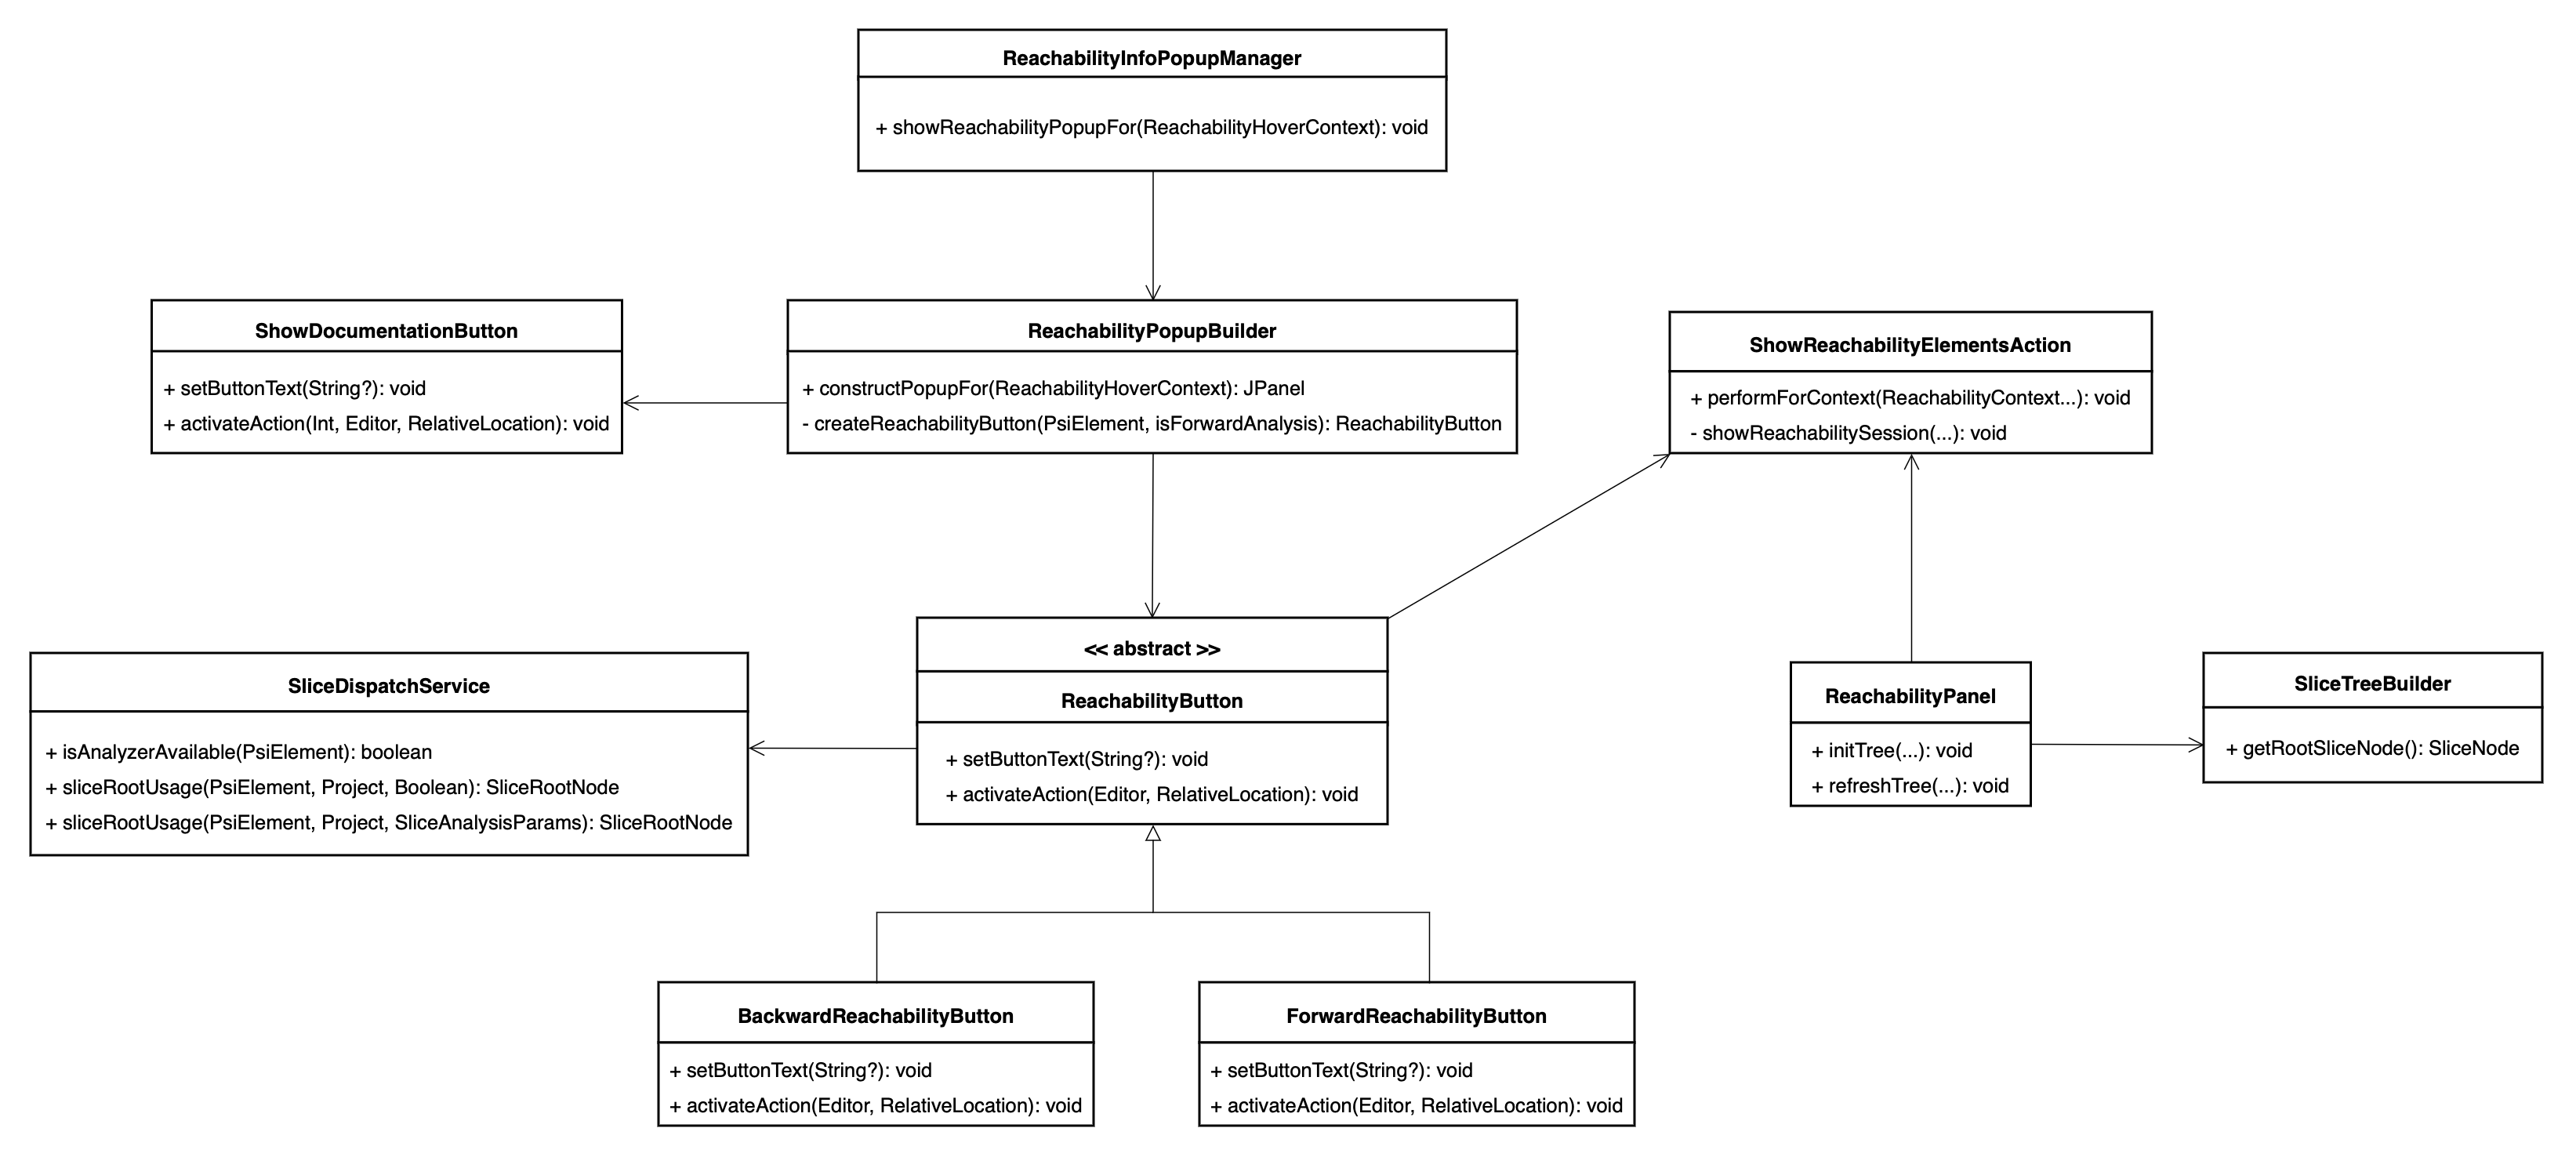
\includegraphics[scale=0.35]{./figs/reach-hover-backend.png}
\caption{
  A simplified architectural diagram of the \toolname{} backend.
}
\label{fig:ReachHoverBackend}
\end{figure}
\end{landscape}

\endinput
